% Created 2023-09-07 Thu 13:39
% Intended LaTeX compiler: pdflatex
\documentclass[11pt]{article}
\usepackage[utf8]{inputenc}
\usepackage[T1]{fontenc}
\usepackage{graphicx}
\usepackage{longtable}
\usepackage{wrapfig}
\usepackage{rotating}
\usepackage[normalem]{ulem}
\usepackage{amsmath}
\usepackage{amssymb}
\usepackage{capt-of}
\usepackage{hyperref}
\usepackage{modiagram, graphicx}
\graphicspath{ {./images/} }
\author{Hankertrix}
\date{\today}
\title{Molecular Orbital Theory Cheat Sheet}
\hypersetup{
 pdfauthor={Hankertrix},
 pdftitle={Molecular Orbital Theory Cheat Sheet},
 pdfkeywords={},
 pdfsubject={},
 pdfcreator={Emacs 29.1 (Org mode 9.6.6)}, 
 pdflang={English}}
\begin{document}

\maketitle
\setcounter{tocdepth}{2}
\tableofcontents

\newpage

\section{Definitions}
\label{sec:orgb4ce093}

\subsection{Constructive interference}
\label{sec:org0ec7e03}
When two wave functions (orbitals) on different atoms \textbf{constructively interfere}, they produce a new molecular orbital that \textbf{promotes} bonding, given by:
\[\Psi(1s)_{H(1)} + \Psi(1s)_{H(2)} \rightarrow \Psi_{b(H-H)}\]

This new molecular orbital has a greater amplitude.

\subsection{Destructive interference}
\label{sec:org07c7abf}
When two wave functions (orbitals) on different atoms \textbf{destructively interfere}, they produce a new molecular orbital that \textbf{decreases} bonding, given by:
\[\Psi(1s)_{H(1)} - \Psi(1s)_{H(2)} \rightarrow \Psi_{b(H-H)}\]

This new molecular orbital has smaller amplitude.

\subsection{Bonding molecular orbitals}
\label{sec:orgae32cda}
The \textbf{addition} of atomic orbitals forms a \textbf{bonding} molecular orbital, which has a region of \textbf{high} electron density between the nuclei. It is given by the \textbf{constructive interference} of two atomic orbitals and expressed by:
\[\Psi_A + \Psi_B \rightarrow \text{Bonding molecular orbital}\]

\subsection{Anti-bonding molecular orbitals}
\label{sec:org0e19ca2}
The \textbf{subtraction} of atomic orbitals forms an \textbf{anti-bonding} molecular orbital, which has a region of \textbf{zero} electron density between the nuclei. It is given by the \textbf{destructive interference} of two atomic orbitals and expressed by:
\[\Psi_A - \Psi_B \rightarrow \text{Anti-bonding molecular orbital}\]

\subsection{HOMO}
\label{sec:org1940191}
HOMO is the highest occupied molecular orbital, which refers to the molecular orbital with the \textbf{highest energy} that is \textbf{occupied} by electrons.

\subsection{LUMO}
\label{sec:org12a8b16}
LUMO is the lowest unoccupied molecular orbital, which refers to the molecular orbital with the \textbf{lowest} energy that is \textbf{unoccupied} by electrons.

\subsection{SUMO}
\label{sec:org2b98b4e}
SUMO is the highest singly occupied molecular orbital, which refers to the molecular orbital with the \textbf{highest energy} that is \textbf{occupied} by electrons, and is also \textbf{singly} filled.

\subsection{Gerade (\(\sigma_g\))}
\label{sec:org328672c}
Gerade refers to molecular orbitals that are symmetric to inversion

\subsection{Ungerade (\(\sigma_u\))}
\label{sec:orgfe709bf}
Ungerade refers to molecular orbitals that are antisymmetric to inversion.

\subsection{Aufbau principle}
\label{sec:orgeef9e58}
Orbitals are filled up in the order of increasing energy.

\subsection{Hund's rule}
\label{sec:orgf004ea5}
Orbitals are first singly filled and pairing starts when more electrons are to be accommodated.

\subsection{Bond order}
\label{sec:org70734fd}
Bond order gives an indication on the number of covalent bonds between the two combining atoms of a molecule. Bond order is given by:
\[\text{Bond order} = \frac{1}{2}(N_b - N_{ab})\]

\(N_b\) refers to the number of electrons in \textbf{bonding} molecular orbitals, while \(N_{ab}\) refers to the number of electrons in \textbf{anti-bonding} molecular orbitals.

\subsection{Paramagnetism}
\label{sec:org45494e2}
Paramagnetism is caused by \textbf{unpaired electrons} in the molecule and results in a strong attraction between the magnetic field and the molecule.

\subsection{Diamagnetism}
\label{sec:orga4a6d67}
Diamagnetism is caused by having \textbf{no unpaired electrons} in the molecule and results in a weak repulsion between the magnetic field and the molecule.


\section{Molecular orbital theory}
\label{sec:orgb99d48a}
Molecule orbital theory is based on the Schr\(\"{o}\)dinger's equation which describe the \textbf{wave properties of electrons} in atoms. This means that understanding superposition will be helpful in understanding molecular orbital theory.


\section{Differences in bonding between the 2 theories}
\label{sec:org3bbc242}

\subsection{Valence bond theory}
\label{sec:org4307f36}
A molecule is viewed as a group of atoms bonded through \textbf{localised overlapping} of valence-shell atomic or hybrid orbitals occupied by electrons.

\subsection{Molecular orbital theory}
\label{sec:org733b329}
A molecule as a collection of nuclei with orbitals \textbf{delocalised over the whole molecule} and occupied by electrons.


\section{Conditions required for bonding}
\label{sec:orgaa81816}
\begin{enumerate}
\item \textbf{Orbital symmetry} must be such that regions with same sign (positive and positive or negative and negative) for the wave function of the electrons to overlap.
\item The \textbf{energies} of the atomic orbitals must be similar.
\item The \textbf{distance} between atoms must be short enough to provide good overlap while being long enough to prevent excessive repulsive forces.
\end{enumerate}

\newpage

\section{Rules of molecular orbital theory}
\label{sec:org6e3364c}
\begin{itemize}
\item Molecular orbitals are constructed by symmetry (orbitals of same sign must be together).
\item Atomic orbitals of similar energy combine more effectively to give molecular orbitals of vastly different energy from the atomic orbitals.
\item Distance between atoms must be short enough to provide good overlap.
\item The number of molecular orbitals must be equal to the total number of atomic orbitals contributed due to the conservation of energy.
\item The bonding molecular orbitals are lower in energy than anti-bonding molecular orbitals. Also, the bonding molecular orbitals are lower in energy and the anti-bonding molecular orbitals are higher in energy than the atomic orbitals that combined to form them.
\item Electrons are assigned to successive higher energy molecular orbitals.
\item The \textbf{addition} of two wave functions represents \textbf{attraction}.
\item The \textbf{subtraction} of two wave functions represents \textbf{repulsion}.
\end{itemize}

\newpage

\section{Why are bonding molecular orbitals lower in energy than anti-bonding molecular orbitals?}
\label{sec:orge6b8da6}
We have to look at the electronic density of the molecular orbital. The electronic density is given by \(\Psi_A^2\).
\\[0pt]

For \textbf{bonding} molecular orbitals, the \textbf{electronic density} is:
\begin{align*}
(\Psi_b)^2 &= (\Psi_A + \Psi_B)^2 \\
&= \Psi_A^2 + \Psi_B^2 + 2 \Psi_A \Psi_B
&< \Psi_A^2 + \Psi_B^2
\end{align*}

This means that the electronic density of the bonding molecular orbitals is \textbf{greater} than the \textbf{sum} of the electronic densities of the individual atoms A and B \((\Psi_A^2 + \Psi_B^2)\).
\\[0pt]

For \textbf{anti-bonding} molecular orbitals, the \textbf{electronic density} is:
\begin{align*}
(\Psi_b)^2 &= (\Psi_A - \Psi_B)^2 \\
&= \Psi_A^2 + \Psi_B^2 - 2 \Psi_A \Psi_B
&< \Psi_A^2 + \Psi_B^2
\end{align*}

This means that the electronic density of the bonding molecular orbitals is \textbf{smaller} than the \textbf{sum} of the electronic densities of the individual atoms A and B \((\Psi_A^2 + \Psi_B^2)\).
\\[0pt]

\[\text{Greater electron density}\]
\[\downarrow\]
\[\text{Greater effective overlap of the orbitals}\]
\[\downarrow\]
\[\text{Greater stability of the molecule}\]
\[\downarrow\]
\[\text{Greater stability means that there is less energy associated with the bond}\]

\section{Drawing molecular orbital diagrams}
\label{sec:orgb06b928}
First, draw the atomic orbitals for the two atoms and fill up the electrons for them.
\\[0pt]

Next, draw the molecular orbitals that are formed between the two atoms, including both the bonding and anti-bonding molecular orbitals.
\\[0pt]

The asterisk (\(\text{*}\)) in \(\sigma^* 1s\) stands for \textbf{anti-bonding} molecular orbitals and is usually called a star. The superscript \(b\) in \(\sigma^{b} 1s\) stands for \textbf{bonding} molecular orbitals.
\\[0pt]

Then, fill up the electrons on the molecular orbitals using the Aufbau principle, Hund's rule and Pauli's exclusion principle to fill up the electrons on the molecular orbitals.

\newpage

\section{Case studies}
\label{sec:org0e4f2d1}

\subsection{\(H_2^+\)}
\label{sec:orgb6a7e75}
Since a normal covalent bond has a bond order of 1, \(H_2^+\) has low bond dissociation energy and large bond length compared to a \(H_2\) atom. Hence, this molecule-ion is only found in low-pressure gas form because it is much more reactive than molecular hydrogen, but it does exist.

\subsection{Does \(Be_2\) exist?}
\label{sec:org2dc50cf}
Drawing the molecular orbital energy diagram:
\\[0pt]

\begin{modiagram}
\atom{left}{1s, 2s = {;pair}}
\atom{right}{1s, 2s = {;pair}}
\molecule{1sMO, 2sMO}

% Labels on the 1s orbitals
\node[yshift=-0.5em, below] at (1sleft) {$1s$};
\node[yshift=-0.5em, below] at (1sright) {$1s$};
\node[yshift=-0.5em, below] at (1sigma*) {$\sigma^* 1s$};
\node[yshift=-0.5em, below] at (1sigma) {$\sigma^b 1s$};

% Labels on the 2s orbitals
\node[yshift=-0.5em, below] at (2sleft) {$2s$};
\node[yshift=-0.5em, below] at (2sright) {$2s$};
\node[yshift=-0.5em, below] at (2sigma*) {$\sigma^* 2s$};
\node[yshift=-0.5em, below] at (2sigma) {$\sigma^b 2s$};
\end{modiagram}
\\[0pt]

Finding the bond order:
\begin{align*}
\text{Bond order} &= \frac{1}{2}(N_b + N_ab) \\
&= \frac{1}{2}(4 - 4) \\
&= 0
\end{align*}

Since the bond order is 0, this means that molecular \(Be\) does not exist as \(Be_2\).

\newpage

\section{\(2s-2p\) orbital mixing}
\label{sec:org244989b}
Due to the relatively small energy gaps between \(2s\) and \(2p\) orbitals in \(B, C, N\) atoms, the \(s-p\) mixing is found in their diatomic molecules. The relatively huge energy gaps between the \(2s\) and \(2p\) orbitals in \(O, F, Ne\) atoms result in \textbf{no} \(s-p\) mixing in their diatomic molecules.
\\[0pt]

When there is \(2s-2p\) orbital mixing, both bonding and anti-bonding \(\sigma_{2s}\) orbitals become lower in energy and both bonding and anti-bonding \(\sigma_{2p}\) orbitals become higher in energy. The \(\sigma_{2p}\) bonding orbitals should have a \textbf{higher energy level} than that of the \(\pi_{2p}\) bonding orbitals.

\[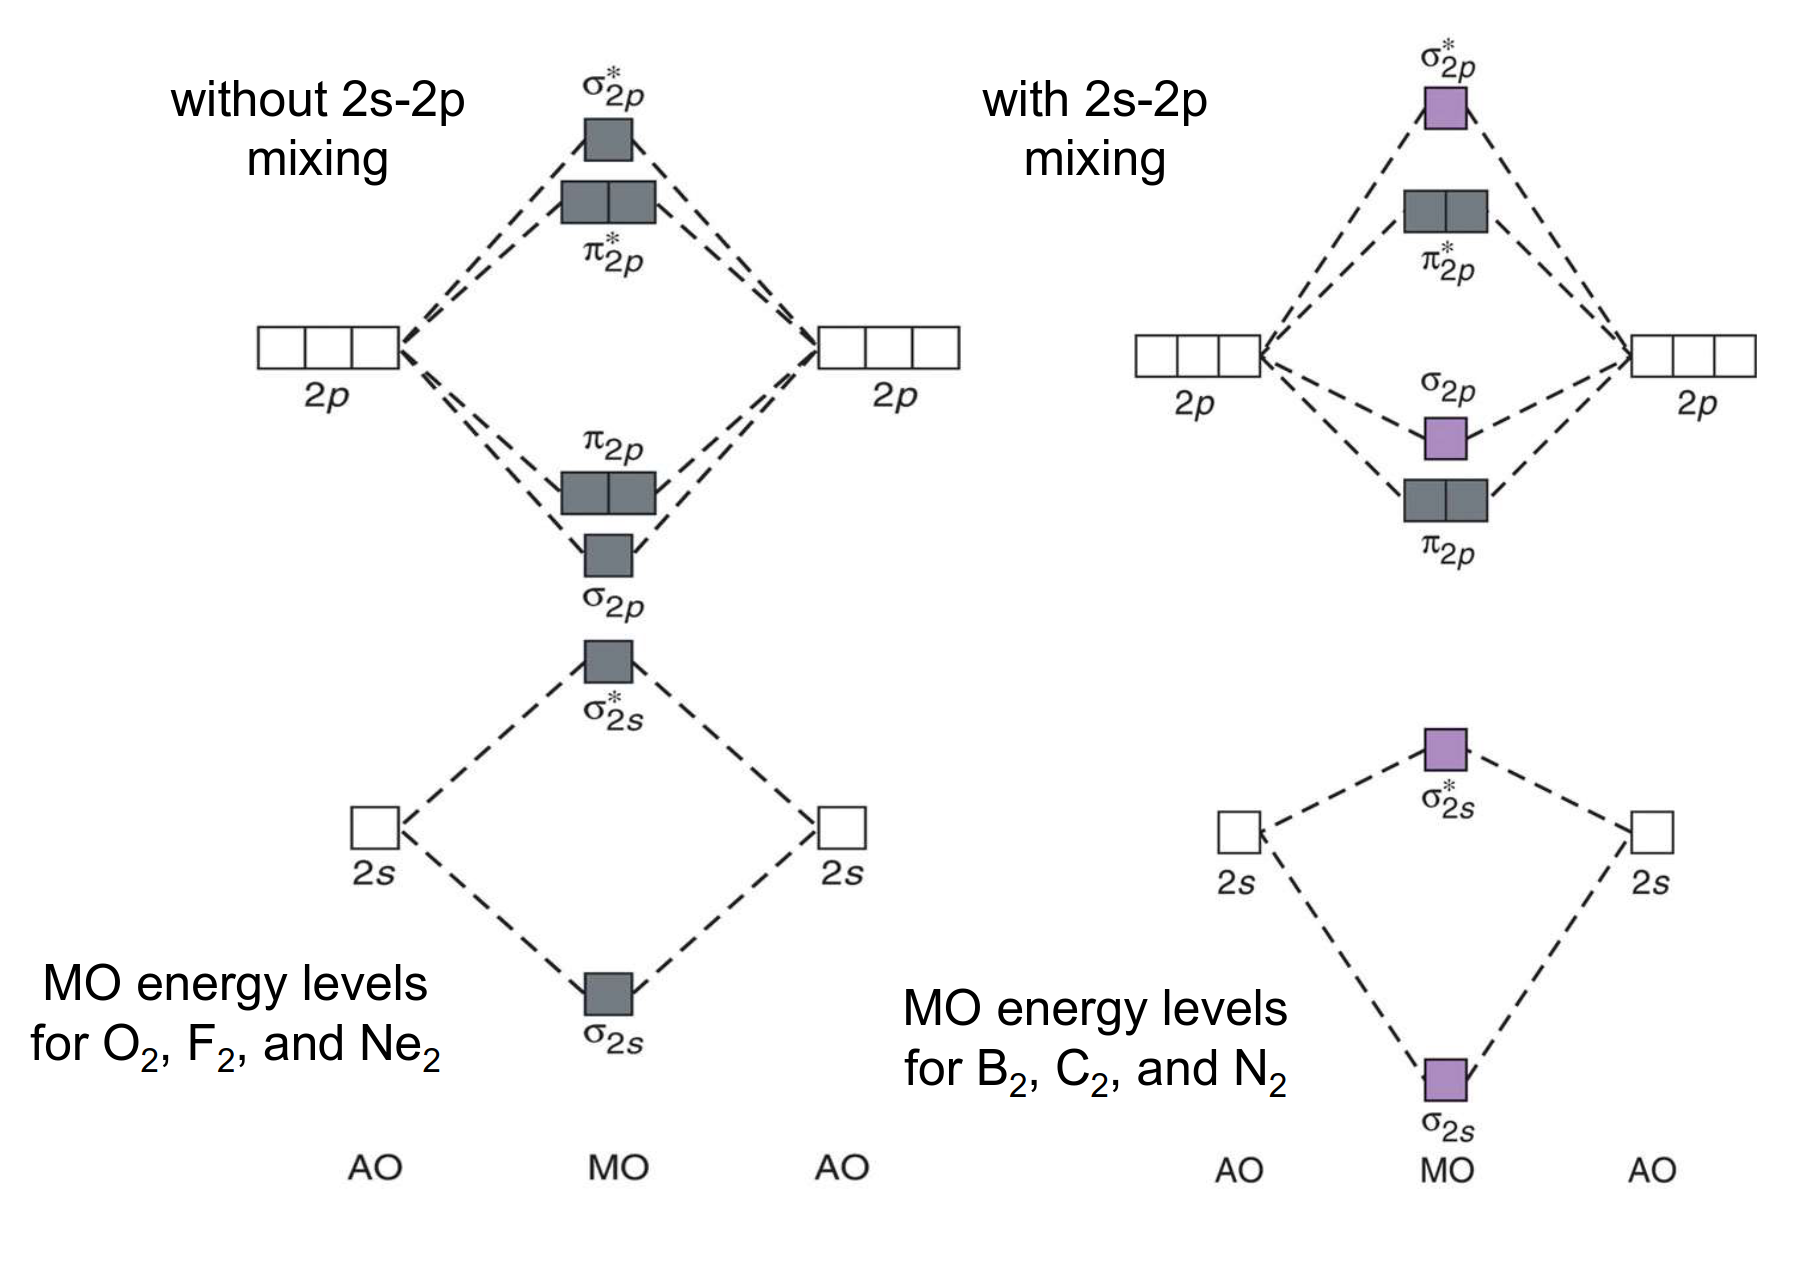
\includegraphics[width = \textwidth]{2s-2p-orbital-mixing}\]

\newpage

\section{How to use molecular orbital theory}
\label{sec:org20c0eb6}
\begin{enumerate}
\item Count the \textbf{total number} of electrons in a molecule
\item Construct the molecular orbital diagram
\item Fill up the electrons in the diagram using Aufbau Principle, Hund's Rule and Pauli's Exclusion principle
\item Count the number of electrons in the bonding and anti-bonding orbitals
\item Calculate the bond order using \(\frac{1}{2} (N_b - N_{ab})\)
\end{enumerate}


\section{2s-2p orbital mixing in heteronuclear diatomic molecules}
\label{sec:orgb88425e}
Examples of heteronuclear diatomic molecules include \(CO\), \(NO\), \(HF\).
\\[0pt]

If the difference in electronegativity is \textbf{large}, there usually will be orbital mixing. Computer models suggest that \(CO\) and \(NO\) will involve orbital mixing.
\\[0pt]

For other cases, it is usually difficult to predict which cases have and which don't have orbital mixing.

\subsection{\(CO\)}
\label{sec:orgae9fa3d}
\[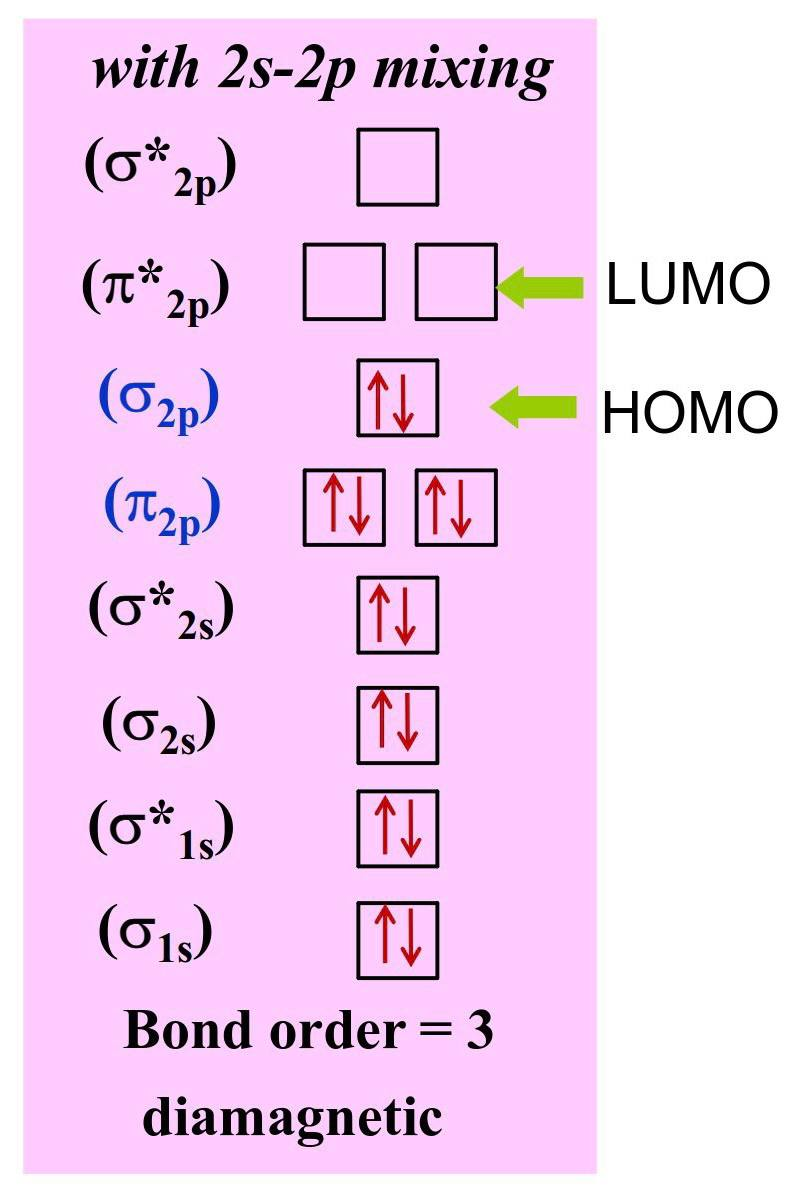
\includegraphics[scale=0.25]{co-molecular-orbital-diagram}\]

\begin{align*}
\text{Bond order} &= \frac{1}{2} (N_b - N_{ab}) \\
&= \frac{1}{2} (10 - 4) \\
&= \frac{1}{2} (6) \\
&= 3
\end{align*}

\subsection{\(NO\)}
\label{sec:org15be8f3}
\[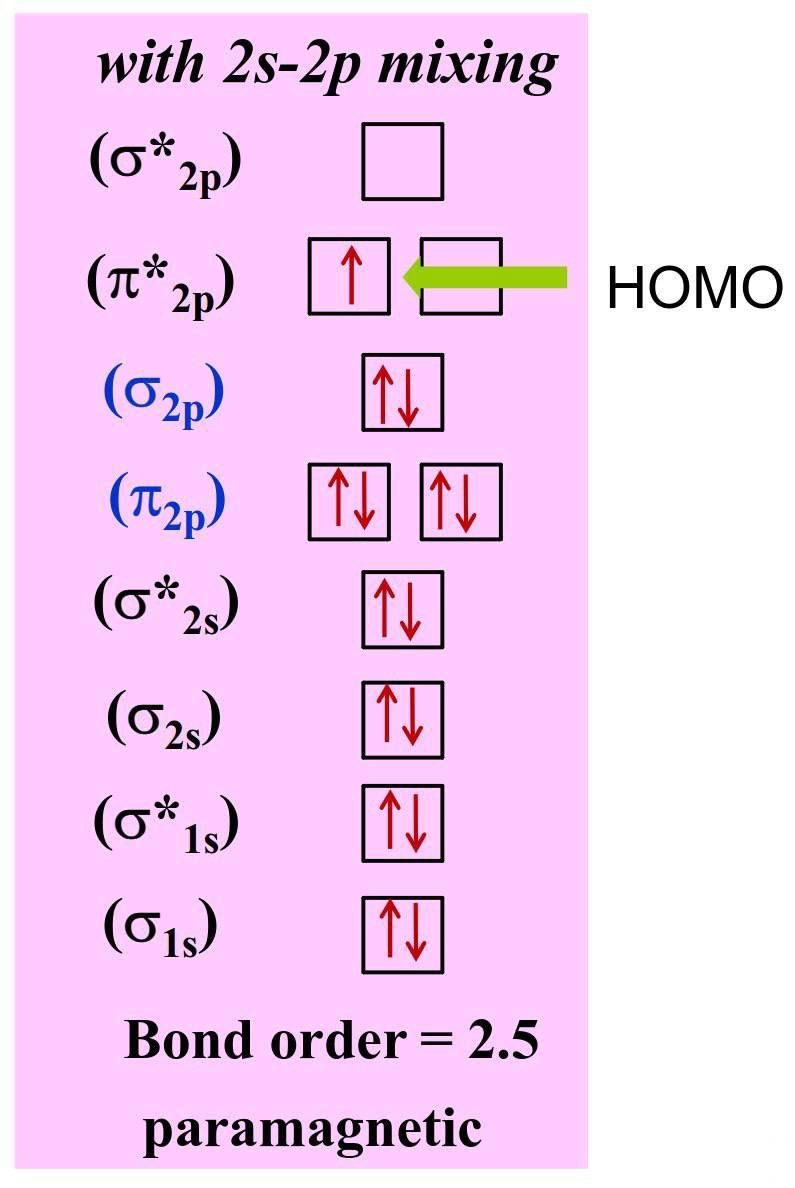
\includegraphics[scale=0.25]{no-molecular-orbital-diagram}\]

\begin{align*}
\text{Bond order} &= \frac{1}{2} (N_b - N_{ab}) \\
&= \frac{1}{2} (10 - 5) \\
&= \frac{1}{2} (5) \\
&= 2.5
\end{align*}

\subsection{\(NO^+\)}
\label{sec:orge8f2931}
\[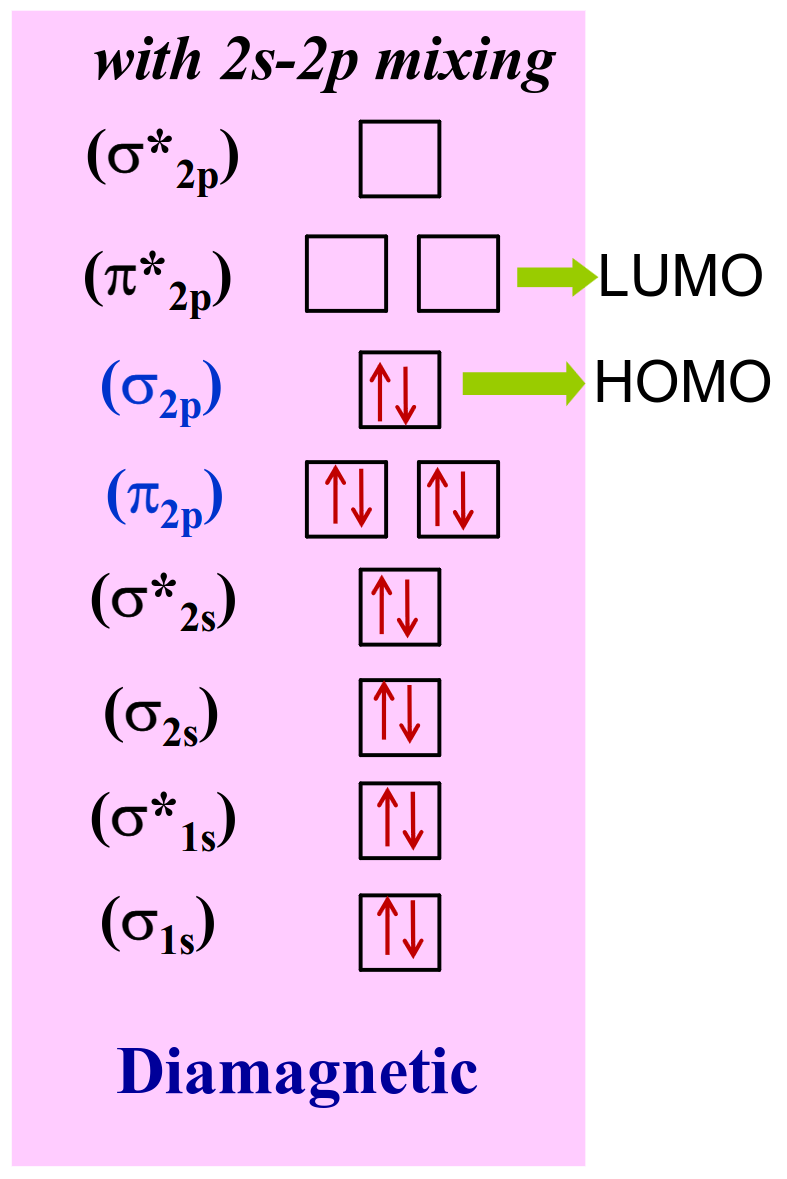
\includegraphics[scale=0.25]{no+-molecular-orbital-diagram}\]

\begin{align*}
\text{Bond order} &= \frac{1}{2} (N_b - N_{ab}) \\
&= \frac{1}{2} (10 - 4) \\
&= \frac{1}{2} (6) \\
&= 3
\end{align*}

\newpage

\subsection{Warning}
\label{sec:orgc9f8f0b}
Heteronuclear diatomic cases are not always simple, as you will see in the later few examples.
\\[0pt]

When two atoms of a diatomic molecule are very different, the energy-level diagram for homonuclear molecules can \textbf{no longer be used}. A \textbf{new} diagram must be devised for each molecule.

\newpage

\subsection{\(HF\)}
\label{sec:orgc03cd33}
Orbital energy between \(H\) and \(F\).
\[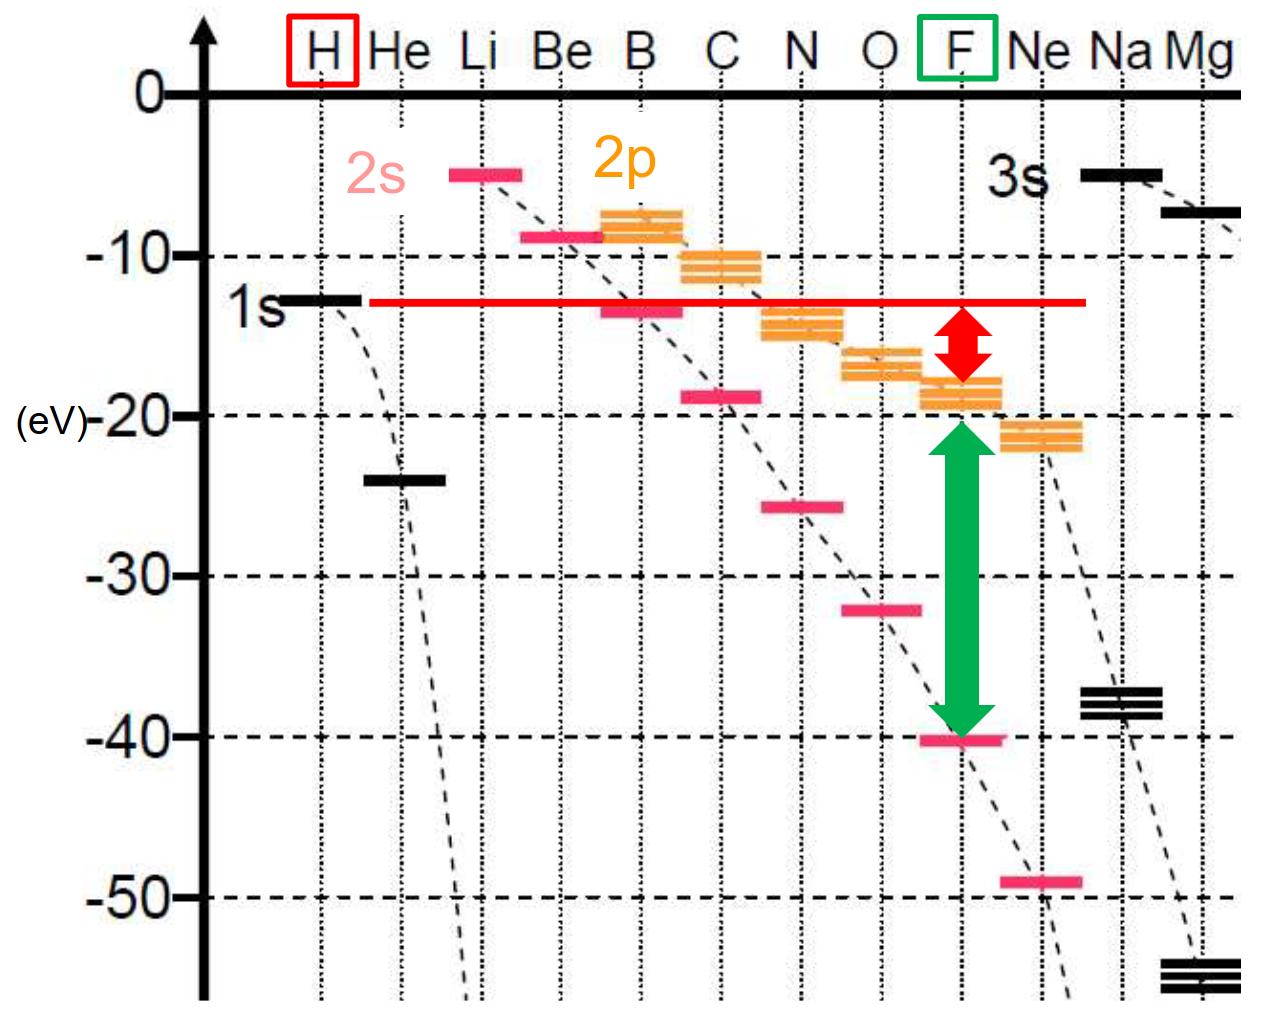
\includegraphics[width = \textwidth]{hf-orbital-energy}\]

The energy difference between the \(1s\) and \(2s\) of \(F\) and \(1s\) of \(H\) is \textbf{too large} for them to interact. Assuming the \(2p_z\) orbital to be the one forming the head-on overlap with the \(1s\) orbital of \(H\), \(2p_x\) and \(2p_y\) do not have the correct orientation to mix with \(1s\) of H. That leaves only \(2p_z\) to interact with the \(1s\) of H, forming a bonding and an anti-bonding orbital. Hence, the remaining \(2p_x\) and \(2p_y\) electrons of \(F\) remain as \textbf{non-bonding molecular orbitals}.

\[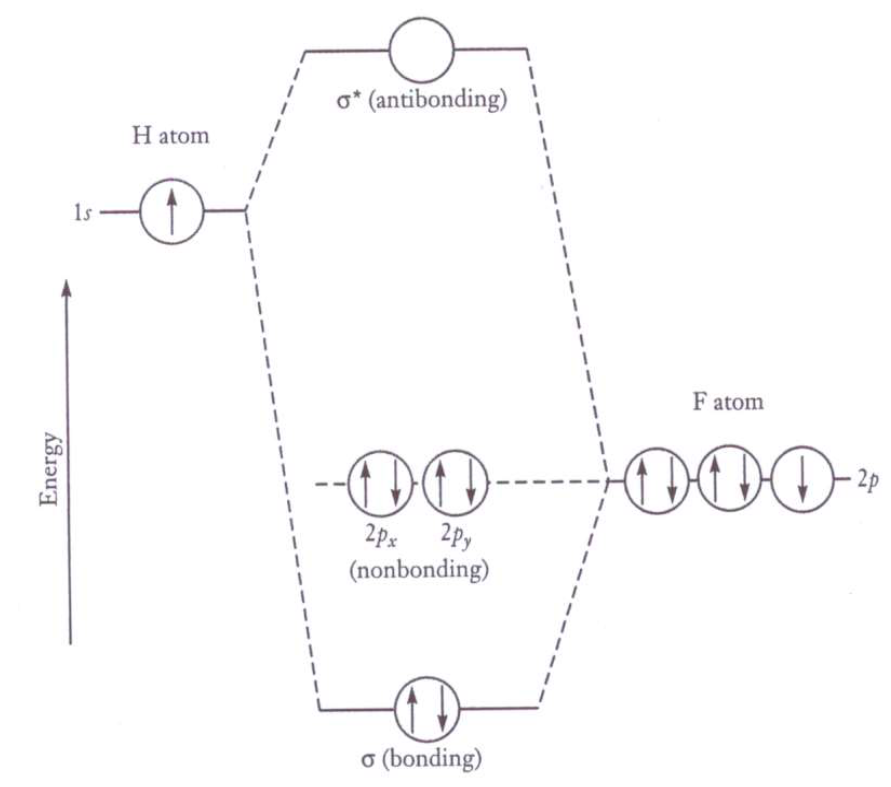
\includegraphics[width = \textwidth]{hf-molecular-orbital-diagram}\]

\begin{align*}
\text{Bond order} &= \frac{1}{2} (N_b - N_{ab}) \\
&= \frac{1}{2} (2 - 0) \\
&= \frac{1}{2} (2) \\
&= 1
\end{align*}

Since there are no lone electrons in the molecular orbitals of \(HF\), \(HF\) is \textbf{diamagnetic}.
\\[0pt]

Since the \(2p\) orbital in \(F\) is lower in energy that the \(1s\) orbital in \(H\), the electrons prefer to be closer to the \(F\) atom which results in greater electron density close to the \(F\) atom.

\subsection{\(LiF\)}
\label{sec:org484fbba}
Orbital energy between \(Li\) and \(F\).
\[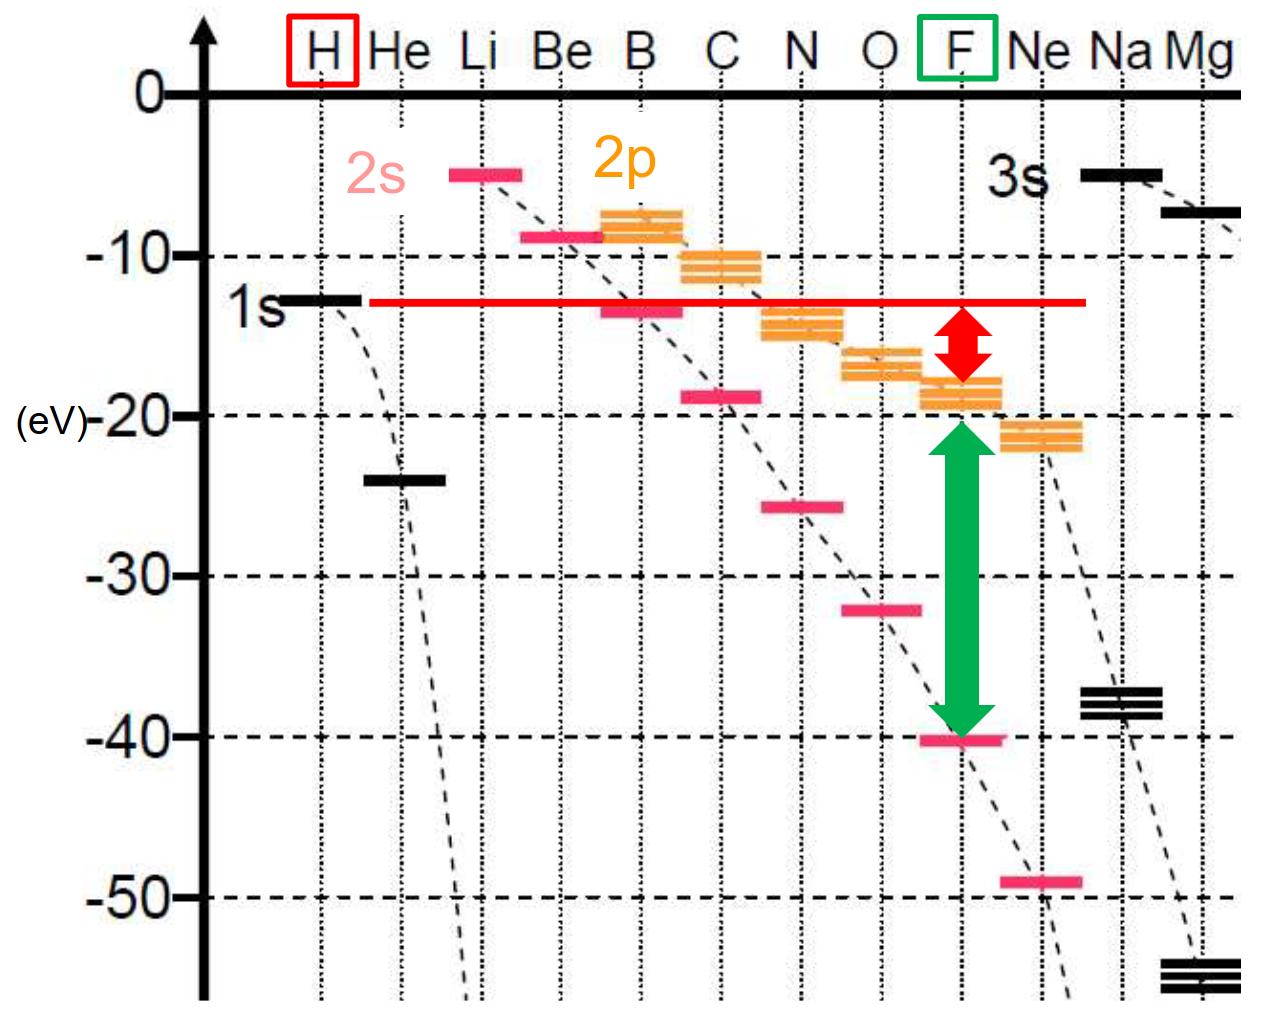
\includegraphics[width = \textwidth]{hf-orbital-energy}\]

The \(2s\) orbital of \(Li\) is higher in energy than both the \(1s\) and \(2s\) orbitals of \(F\). Hence, \(Li\) only interacts with \(2p_z\) orbital of \(F\) and all remaining electrons in \(F\) are in \textbf{non-bonding molecular orbitals}.

\[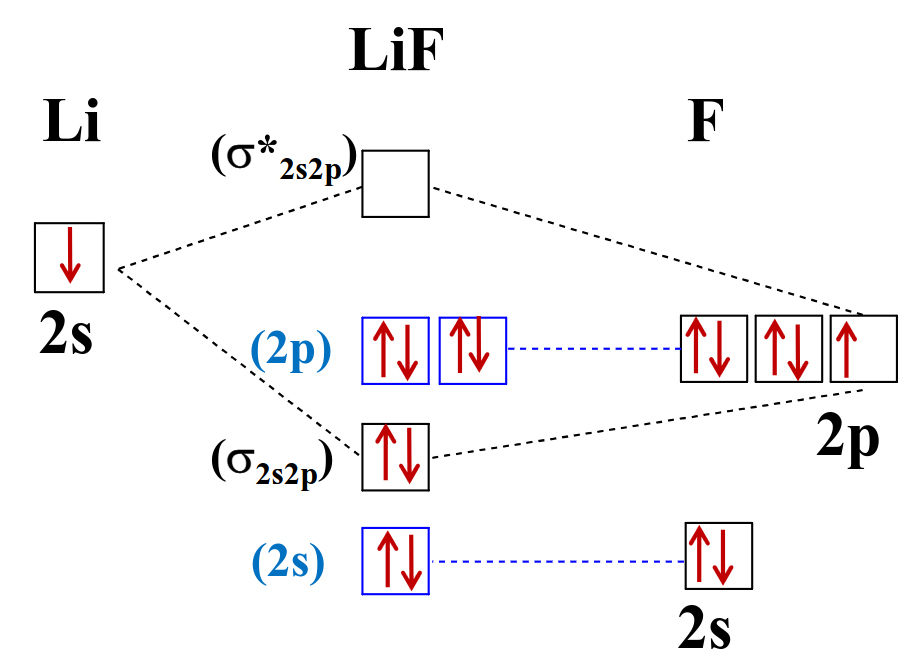
\includegraphics[width = \textwidth]{lif-molecular-orbital-diagram}\]

\begin{align*}
\text{Bond order} &= \frac{1}{2} (N_b - N_{ab}) \\
&= \frac{1}{2} (2 - 0) \\
&= \frac{1}{2} (2) \\
&= 1
\end{align*}

Since there are no lone electrons in the molecular orbitals of \(LiF\), \(LiF\) is \textbf{diamagnetic}.

\newpage

\subsection{\(OH^-\)}
\label{sec:orga10475b}
The \(1s\) orbital of \(O\) is higher in energy than both the \(1s\) and \(2s\) orbitals of \(O\). Hence, \(O\) only interacts with the \(2p_z\) orbital of \(O\) and all remaining electrons in \(O\) are in \textbf{non-bonding molecular orbitals}.

\[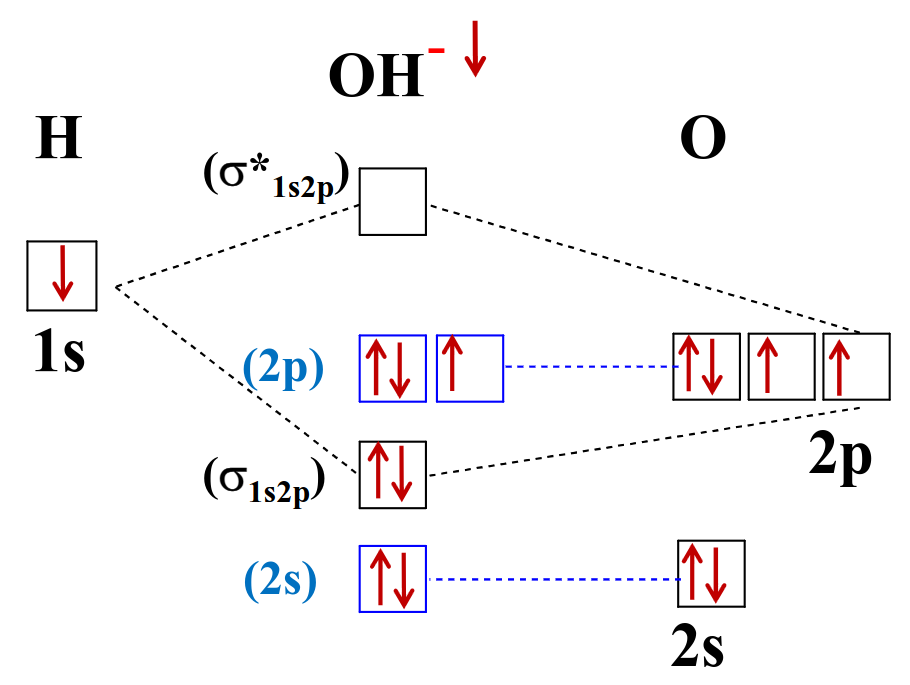
\includegraphics[width = \textwidth]{oh--molecular-orbital-diagram}\]

\begin{align*}
\text{Bond order} &= \frac{1}{2} (N_b - N_{ab}) \\
&= \frac{1}{2} (2 - 0) \\
&= \frac{1}{2} (2) \\
&= 1
\end{align*}

Since there are no lone electrons in the molecular orbitals of \(OH\), \(OH\) is \textbf{diamagnetic}.
\end{document}